\documentclass[version=last,fontsize=13pt]{scrartcl}


\usepackage{pdfpages}
\usepackage{graphicx}
\usepackage{indentfirst}

\usepackage{titlesec}
\usepackage{caption}

\titlespacing*{\section}{0pt}{3ex}{3ex}
\titlespacing*{\subsection}{0pt}{1.5ex}{1.5ex}
\titlespacing*{\subsubsection}{0pt}{1.5ex}{1.5ex}

\usepackage[margin = 0.8in]{geometry}

% dont number sections
\setcounter{secnumdepth}{0}

\usepackage{wrapfig}
\usepackage{float}

\usepackage{caption}
\usepackage{subcaption}

\usepackage{tabularx}
\begin{document}

\begin{titlepage}
	\begin{center}	
		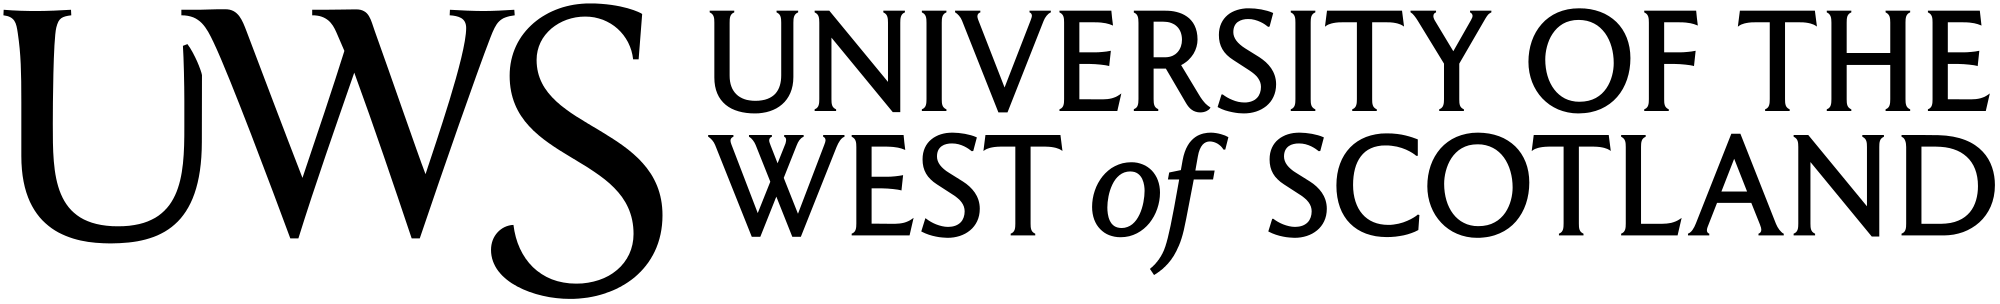
\includegraphics[width = 5cm,height = 1.5cm]{./imgs/uws_logo.png}\\[5cm]
	
	 { \huge \bfseries %
		How can Android Packed malware be detected and prevented?\\} 

	\vspace{6cm}			
			
		\begin{flushright}
				\large Student:\\
				Marius-Lucian Olariu\\[1cm]
		\end{flushright}
		
	
		\begin{flushleft}
			 \large
				Supervisor: \\
				Dr. Zeeshan Pervez \\[1cm]
		\end{flushleft}
		
	\vspace{2cm}	
	
		
		\vfill

			{\large {Paisley \\ 2019}}
		\end{center}
\end{titlepage}

\newpage

\tableofcontents

\newpage

\listoffigures

\listoftables

\newpage


\section{Introduction}(5p - 500w)\\


%add information from the presentation slides and speakers notes

%summarise the traditional packaging technique
	Android is an \textbf{O}perating \textbf{S}ystem (OS) designed for mobile devices like tablets and smartphones and is currently the market leader  of mobile operating systems since of 2016 (Mobile OS Market Share 2018, 2019). Android has been the leading mobile OS in phones sold since 2011 as can be seen in Figure~\ref{aStats} (Mobile OS Market Share 2018, 2019). The CEO of Google, Sundar Pichai, declared at Google I/O 2017 that there are over two billion smartphones running Android OS  (Google I/O 2017, n.d). The success of Android is due to the fact that is very efficient (uses a modified version of the Linux kernel) and open-source.  The fact that Android is open-source and the large number of users it has attracts a lot of attackers to develop malware (huge material gains and prestige). The problem of Android malware is similar to the one Windows OS faces, in other words, because most of the personal computers run Windows most of the  malware targets Windows systems and not Linux or macOS systems. Another fact that makes Android so appealing to malware authors is the fact that is very easy to install applications from unknown sources and  there are many third-party markets for distribution of  Android applications.\\ 

	\begin{figure}[H]

		\caption{Global market share sales by mobile OSs from 2009 to 2018}
		\label{aStats}

		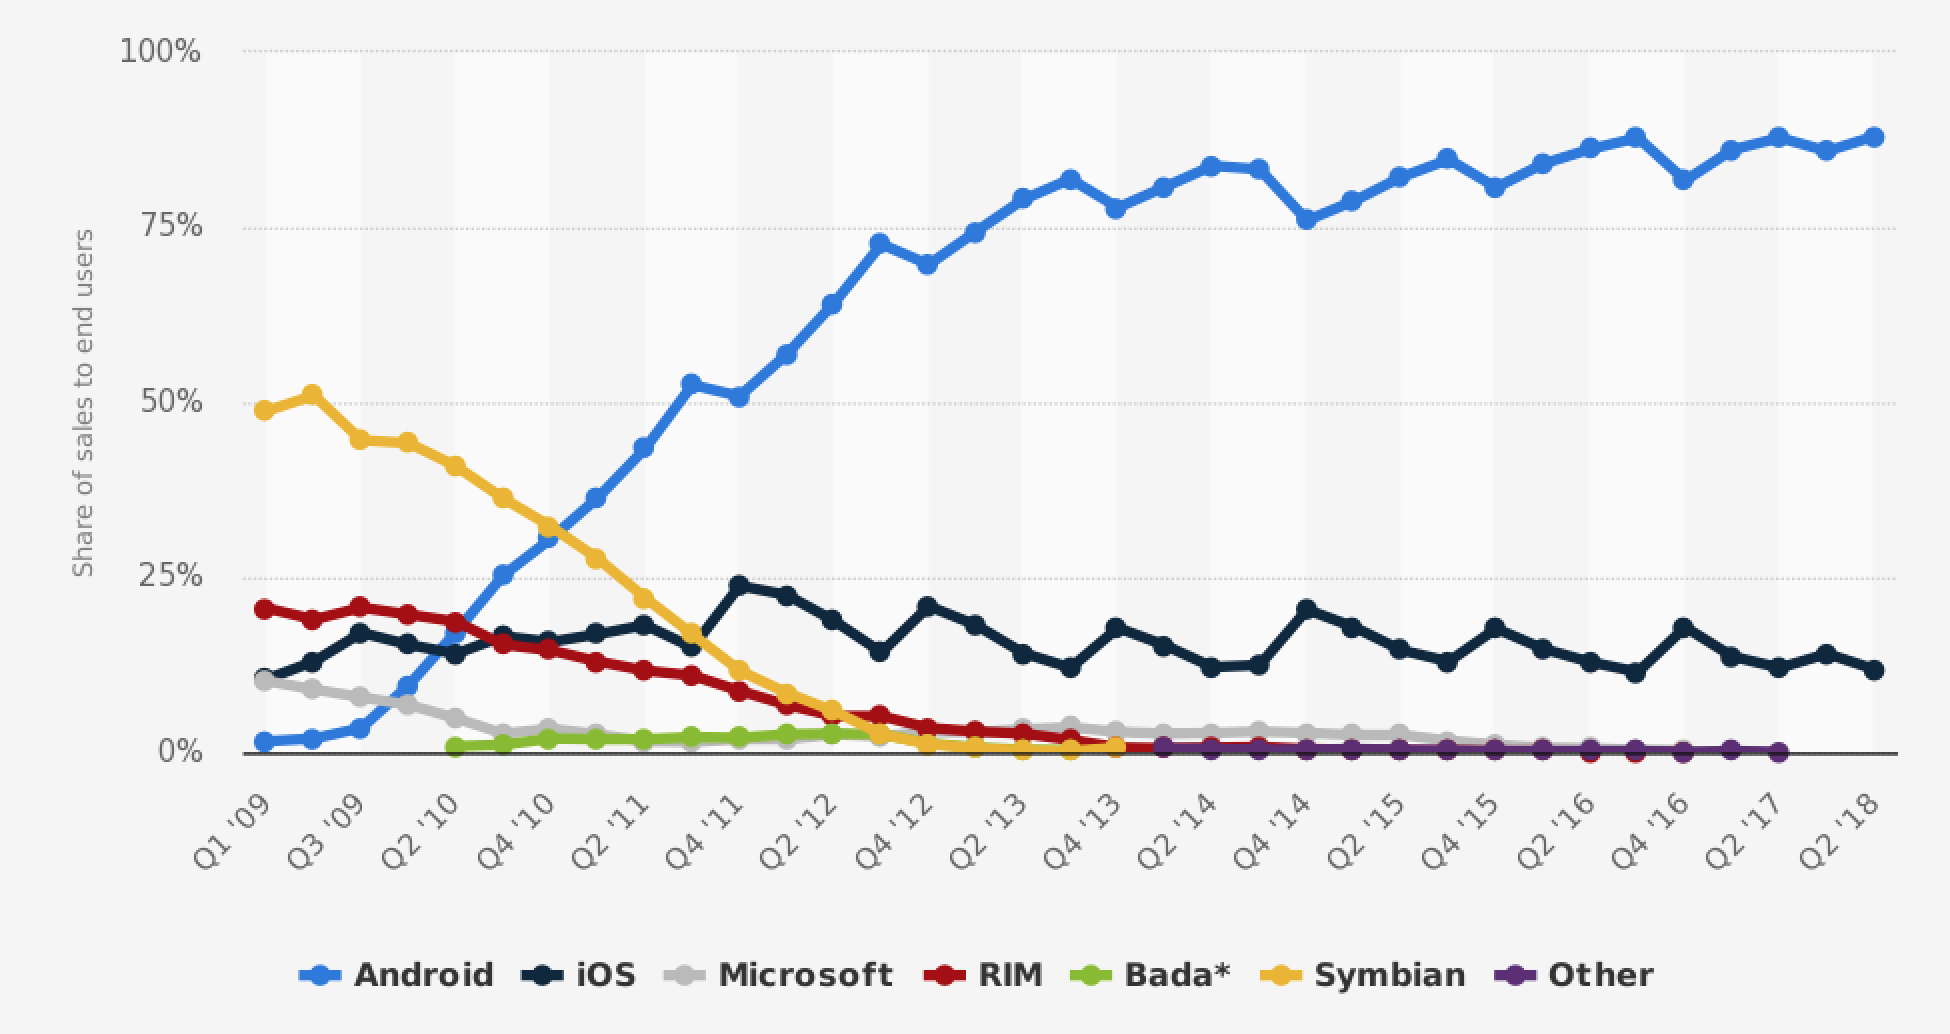
\includegraphics[scale = 0.48]{./imgs/androidStats.png}
	\end{figure}
	
	\indent
	Android applications are distributed and installed using the \textbf{A}ndroid \textbf{P}ac\textbf{k}age (.apk) format. The apk format is essentially an archive (was extended from JAR and ZIP) that contains the application compiled code, resources, certificates and the manifest file. Because an apk file it is just an archive it can be easily unarchived, thus it a fairly straight process to get to the complied code of a certain application once you have the apk file. For Android the compiled code is in \textbf{D}alvik \textbf{Ex}ecutable (DEX) format and because executable code is hard to understand for a human it needs to be further converted. DEX files can be converted to a human-readable format known as \textit{smali} using open-source tools like \textit{Apktool} (Tumbleson, n.d.). Moreover, \textit{Apktool} recovers the xml files and Android manifest file to a form close to the orignal ones. Typically, a smali file coresponds to a Java class code. In order to add malicious code the attacker can add smali code in the app files or add new smali files containg malicious code. For instance one could write a broadcast receiver that reads and sends the phone contacts of the users to a webserver and is triggered when the user restarts his phone, this does not need too much effort from an attacker. Once the malicious code is added to the application, the attacker reasembles everything again into an apk file (representing the malicious Android app). The next step is to sign the newly created apk file which can be done either using an certificate authority or a private key generated by the attacker of the app, obviously the attacker will pick the later variant. The signing of an apk file should help Google identify the author of an application, however, non-official markets are not really interested in finding the author of an app. At this point the attacker has "cloned" a genuine app and is free to redistribute it.  In short,  the above described process is known as the \textit{repackaging attack}, please see Figure~\ref{repA} for a visual depiction of the attack (Wenliang, 2015) .\\

	\begin{figure}[H]
		\centering
		\caption{Overview of the repackaging attack}
		\label{repA}

		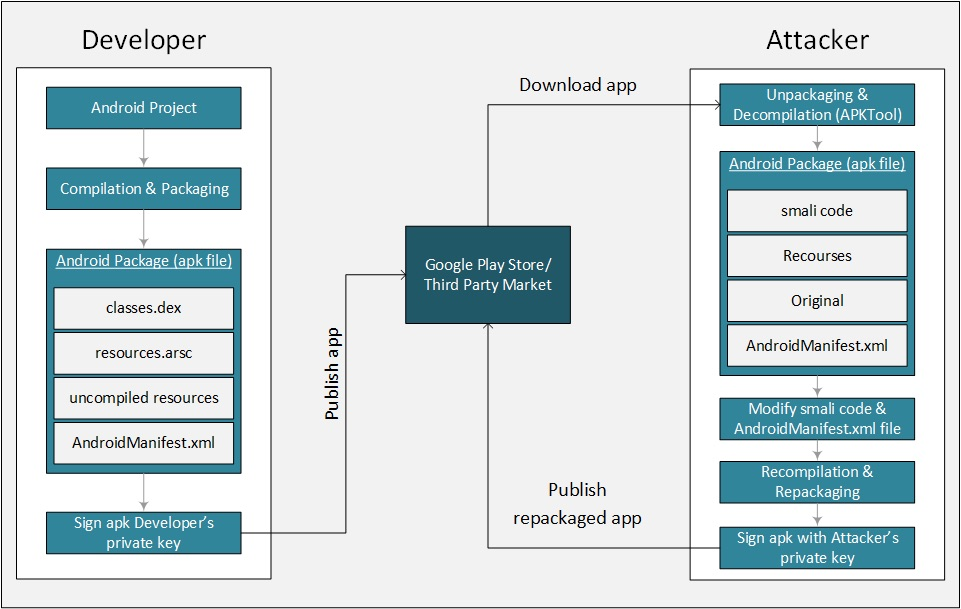
\includegraphics[scale = 0.50]{./imgs/repackAttack}
	\end{figure}
	
	
	\indent
	In order to overcome the above mentioned attack there have been developed Android Packers that can enhance Android applications by providing anti-decompliation, anti-runtime injection and anti-debug techniques. The Android Packers are available only through  where the developer can upload his apk file and get it in \textit{packed} form which is safer for distribution on application markets.  However, recently the Android Packers have started to be used not only by developers to protect their intelectual property but also by hackers to better hide malware in applications (Yang et al, 2015).  A packed application  poses a real challenge for cybersecurity specialists because it is really hard to be analyzed to detect if is bening or malicious.  


\section{Literature review}(10p - 1000w)\\

\subsection{DroidUnpack}
	DroidUnpack is a framework developed for detection and analysis of Android applications with packed malware and it can monitor app execution at the lowest level and also reconstruct Java level execution (Duan et al., 2018). In other words, DroidUnpack is an emulator that can run the Android OS with the app to be analysed and monitors the memory writes performed by the application. The framework has been tested against 93910 Android applications containing malware, 6 major commercial packers (Ali, Baidu, Bangle, Ijami, Qihoo and Tencent) and 3 unpackers (DexHunter, AppSpear and Kisskiss) over a large time frame (2010 - 2015) and the authors want to make it public in the future.\\
	DroidUnpack makes use of the following tools to analysis tools to investigate a packed application:

	\begin{itemize}
		\item The Hidden Code Extractor
		\item The Multi-layer Unpacking Detector
		\item The Self-Modifying Code Detector
		\item The JNI inspector
	\end{itemize}

	For a general view of the framework please see Figure~\ref{droid}.

	\begin{figure}[H]
		\centering
		\caption{Overview of the DroidUnpack framework}
		\label{droid}

		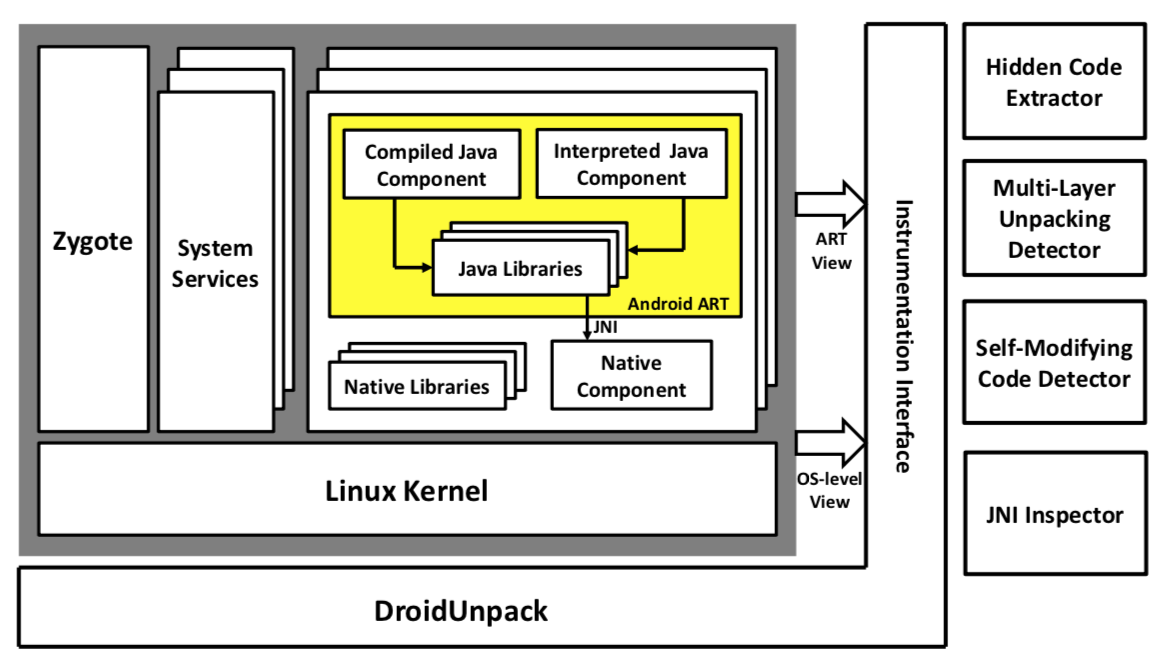
\includegraphics[scale = 0.8]{./imgs/droidUnpack}
	\end{figure}
	
\subsection{DexHunter}


\section{Security and privacy advancement and glitches} (10p - 1000w)


\section{Real-world scenarios, use cases}(8p - 800w)\\
%examples to demonstrate the impact
%talk about DroidDream Trojan
%Zeus
%SMSSend
%talk about Obfuscated Malware discovered on google Play
\section{Conclusion}(5p - 500w)\\


\pagebreak
\section{References}

\underline{Defining Malware: FAQ.} (2019) [Online] Available: https://docs.microsoft.com/en-us/previous-versions/tn-archive/dd632948(v=technet.10) [Accessed: 6 March 2019].\\

Duan, Y., Zhang, M., Bhaskar, A.V., Yin, H., Pan, X., Li, T., Wang, X. and Wang, X. (2018)\\ \underline{Things you may not know about android (un) packers: a systematic study based on whole-system emulation} In 25th Annual Network and Distributed System Security Symposium, NDSS (pp. 18-21).\\

\underline{Google I/O 2017.} (n.d.) [Online] Available: https://bit.ly/2CvBOjd [Accessed: 12 March 2019].\\

\underline{Mobile OS Market Share 2018.} (2019) [Online] Available: https://bit.ly/2Fwii8f [Accessed: 24 March 2019].\\

Ruiz, F. (2016) \underline{Obfuscated Malware Discovered On Google Play} [Online]  Available: https://bit.ly/2UcWx5y [Accessed: 12 March 2019].

Tumbleson, C. (n.d.) \underline{Apktool.} [Online] Available: https://ibotpeaches.github.io/Apktool/ [Accessed: 24 March 2019].\\

Wenliang, D. (2015) \underline{Android Repackaging Attack Lab} [Online]\\ Available: https://bit.ly/2urlfRa  [Accessed: 24 March 2019]\\

Yang, W., Zhang, Y., Li, J., Shu, J., Li, B., Hu, W. and Gu, D. (2015)\\ \underline{Appspear: Bytecode decrypting and dex reassembling for packed android malware}. In International Workshop on Recent Advances in Intrusion Detection (pp. 359-381). Springer, Cham.\\

\end{document}

